\item Una barra de largo \(L\) y masa \(M_B\), se encuentra unida al extremo de una golilla de radio interno \(r\), radio externo \(R\), masa \(M_G\) y espesor despreciable. Usted consta de dos sistemas de p\'endulo, uno que oscila de frente a usted (esquema 1), que no siente el roce, y otro que oscila de costado a usted (esquema 2), que siente el roce del aire solo en la golilla. Ambos p\'endulos tienen unido a su extremo dos resortes de constantes el\'asticas \(k_1\) y \(k_2\), tal como muestra la figura. Usted debe determinar la potencia promedio de una fuerza arm\'onica externa resonante al sistema, aplicada en el centro de la golilla para el sistema 2.
		\begin{center}
			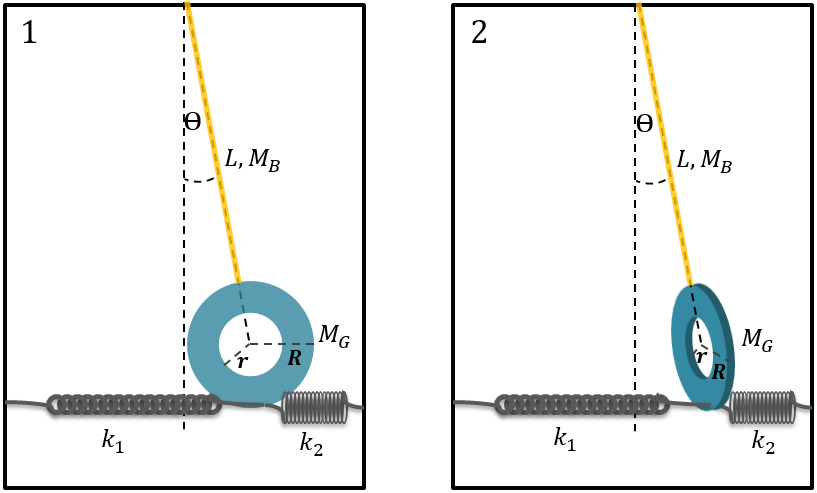
\includegraphics[height=7cm]{Preguntas/images/control1.png}
		\end{center}
		
	\begin{enumerate}[a)]
		\item Determine el momento de inercia respecto al pivote del p\'endulo f\'isico para ambos sistemas \(I_1\) e \(I_2\), en t\'erminos de \(M_B\), \(M_G\), \(R\), \(r\) y \(L\). Los momentos de inercia para un disco de masa \(M\) y radio \(R\) y para una barra de masa \(M\) y largo \(L\) son:
		\begin{center}
			\includegraphics[height=4.5cm]{Preguntas/images/ayuda.png} \hspace{20mm} 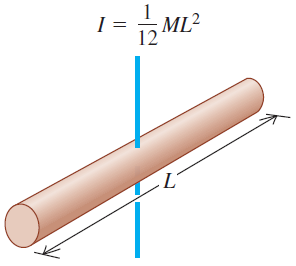
\includegraphics[height=4.5cm]{Preguntas/images/ayuda2.png}
		\end{center}
		\item Determine la frecuencia angular \(\omega_{01}\) para el primer p\'endulo, que no siente roce, en t\'erminos de las variables del problema.
		\item Usted se da cuenta que la frecuencia angular para el segundo p\'endulo es igual que la frecuencia natural del primero, \(\omega_2 = \omega_{01}\). Determine el valor de la constante \(b\) de la fuerza de roce \(\vec{f}_r=-b\dot{\vec{x}}\) para el segundo p\'endulo, considerando que act\'ua en el centro de la golilla. Entregue su resultado en t\'erminos de \(I_1\), \(I_2\), \(k_1\), \(k_2\), \(M_G\), \(M_B\), \(R\), \(r\) y \(L\).
		
		\fbox{Ayuda: \(\omega_2 = \sqrt{\omega_{02}^2 - \gamma^2}\)}

		
		\item \textquestiondown Cu\'anto ser\'ia la potencia promedio \(\bar{P}\), de una fuerza arm\'onica externa resonante con el sistema, \(\vec{F}_0 \cos(\Omega_R t)\), si act\'ua en el centro de la golilla?
		\begin{equation*}
			\bar{P} = \dfrac{1}{T} \int_0^T P \ dt \hspace{10mm} (T \equiv \text{periodo})
		\end{equation*}
		
		\fbox{Ayuda: \(\sin(a \pm b) = \sin (a) \cos(b) \pm \cos (a) \sin (b)\)}
		
		\fbox{Ayuda: \(\phi_2 = \arctan \left( \dfrac{2 \gamma \Omega }{\Omega^2 - \omega_0^2} \right)\)}
		
		
	\end{enumerate}


\textbf{\underline{Soluci\'on:}}

\begin{enumerate}[a)]

\item
	El momento de inercia de la barra respecto al pivote en los dos esquemas aplicando Teorema de Steiner est\'a dado por:
	\begin{equation*}
	I_\text{barra} =\frac{1}{3}M_{\text{B}}L^2
	\end{equation*}
	
	El momento de inercia de la golilla respecto al pivote para el esquema 1 aplicando Teorema de Steiner est\'a dado por:
	\begin{equation*}
	I_\text{golilla,1} = I_\text{CM,1} + M_{\text{G}}{(L+R)}^2
	\end{equation*}
	
	El momento de inercia de la golilla respecto a su centro de masa corresponde a una resta de momentos de inercia, es decir:
	\begin{equation*}
	I_{\text{CM,1}}=\frac{1}{2}M_1R^2-\frac{1}{2}M_2r^2
	\end{equation*}
	
	\noindent donde las masas $M_1$, $M_2$ y $M_\text{G}$ tienen la misma densidad superficial $\sigma$, es decir:
	\begin{equation*}
		\sigma=\frac{M_{\text{G}}}{\pi(R^2-r^2)} = \frac{M_1}{\pi R^2} =\frac{M_2}{\pi r^2}
	\end{equation*}

	Relacionando las masas $M_1$, $M_2$ y $\sigma$ con la masa de la golilla $M_\text{G}$ se obtiene el momento de inercia de la golilla respecto al centro de masa:
	\begin{equation*}
	I_{\text{CM}1}=\frac{1}{2}M_{\text{G}}(R^2+r^2)
	\end{equation*}
	
	Por lo tanto, el momento de inercia del sistema barra-golilla para el esquema 1 es:
	\begin{equation*}
		I_1=\frac{1}{3}M_{\text{B}}L^2 + \frac{1}{2}M_{\text{G}}(R^2+r^2) + M_{\text{G}}{(L+R)}^2
	\end{equation*}
	
	De manera similar, el momento de inercia del esquema 2, $I_2$, es:
	\begin{equation*}
	I_2=\frac{1}{3}M_{\text{B}}L^2 + \frac{1}{4}M_{\text{G}}(R^2+r^2) + M_{\text{G}}{(L+R)}^2
	\end{equation*}
\item
	Para el sistema barra-golilla existen cuatro fuerzas que realizan torque respecto al pivote, dos fuerzas de peso y dos fuerzas del resorte. El torque respecto al pivote es:
	\begin{align*}
		I_1 \ddot\theta &= \Sigma \tau \\
		I_1\ddot\theta &= -M_{\text{B}} g  \frac{L}{2}\sin\theta - M_{\text{G}}g(L+R)\sin\theta - k_1S(L+2R)\cos\theta - k_2S(L+2R)\cos\theta
	\end{align*}
	
	Utilizando que la relaci\'on entre el arco y el \'angulo es $S=(L+2R)\theta$ y aplicando aproximaciones para \'angulos peque\~nos $\sin\theta\approx\theta$ y $\cos\theta\approx1$ se determina la siguiente ecuaci\'on de movimiento:
	\begin{equation*}
	\ddot\theta + \left( \frac{M_{\text{B}}g\frac{L}{2} + M_{\text{G}}g(L+R) + (k_1+k_2){(L+2R)}^2}{I_1}\right) \theta = 0
	\end{equation*}
	
	La frecuencia angular $\omega_{01}$ para el primer p\'endulo es:
	
	\begin{equation*}
		\omega_{01}=\sqrt{\frac{M_{\text{B}}g\frac{L}{2} + M_{\text{G}}g(L+R) + (k_1+k_2){(L+2R)}^2}{I_1}}
	\end{equation*}

\item Utilizando la ayuda obtenemos la relaci\'on $\omega_2=\sqrt{\omega_{02}^2-{\gamma}^2}=\omega_{01}$. De forma similar que para el esquema 1, obtenemos que la ecuaci\'on de movimiento est\'a dada por:
	\begin{equation*}
	\ddot\theta + 2 \gamma \dot\theta + \omega_{02}^2 \theta = 0
	\end{equation*}
	
	\noindent donde la frecuencia natural de oscilaci\'on $\omega_{02}$ del esquema 2 est\'a dada por:
	\begin{equation*}
	\omega_{02} = \sqrt{\frac{M_{\text{B}}g\frac{L}{2} + M_{\text{G}}g(L+R) + (k_1+k_2){(L+2R)}^2}{I_2}}
	\end{equation*}
	
	Se cumplen la siguiente relaci\'on entre las frecuencias naturales y los momentos de inercia entre los dos esquemas: $\omega_{01}^2I_1=\omega_{02}^2I_2$.
	
	Utilizando la ayuda y reemplazando los valores de las frecuencias naturales se obtiene el valor de $\gamma$:
	\begin{gather*}
		\gamma^2=\omega_{02}^2-\omega_{01}^2\\
		{\gamma}^2= \frac{1}{4}M_{\text{G}}\left( R^2+r^2 \right) \left( M_{\text{B}}g\frac{L}{2} + M_{\text{G}}g(L+R) + (k_1+k_2){(L+2R)}^2 \right) \frac{1}{I_1I_2}
	\end{gather*}

	Para determinar la relaci\'on entre $b$ y $\gamma$ debemos determinar el torque de la fuerza de roce respecto al pivote, $\tau_{\text{roce}}=-b\dot x (L+R)\cos\theta$. La relaci\'on entre el arco y el \'angulo para la fuerza de roce es:
	\begin{align*}
		x&=(L+R)\theta\\
		\dot x&= (L+R)\dot\theta
	\end{align*}

	A partir de la ecuaci\'on de movimiento podemos relacionar el torque de la fuerza de roce con el factor $\gamma$, es decir:
	\begin{align*}
		- 2\gamma I_2 \dot \theta&= \tau_{\text{roce}} \\
		- 2\gamma I_2 \dot \theta &= - b (L+R)^2 \dot \theta \cos \theta\\
		b&=\frac{2\gamma I_2}{{(L+R)}^2}
	\end{align*}
	
	Por lo tanto, el valor de la constante $b$ en funci\'on de las variables del sistema es:
	\begin{equation*}
	b= \frac{1}{{(L+R)}^2} \ \sqrt{\frac{I_2}{I_1}} \ \sqrt{ M_{\text{G}}\left( R^2+r^2 \right) \left( M_{\text{B}}g\frac{L}{2} + M_{\text{G}}g(L+R) + (k_1+k_2){(L+2R)}^2 \right) }
	\end{equation*}
	
\item Considerando r\'egimen estacionario, la soluci\'on est\'a dada por:
	\begin{align*}
		x(t) &= A_2\cos (\Omega t + \phi_2) \\
		\dot x (t) &= A_2 \Omega \sin (\Omega t + \phi_2)
	\end{align*}

	La potencia instant\'anea de la fuerza externa est\'a dada por:
	\begin{align*}
		P(t) &= \vec{F}_{\text{ext}} \cdot \dot{\vec{x}} \\
	    P(t) &= A_2 \Omega F_0 \cos(\Omega t) \sin (\Omega t + \phi_2)
	\end{align*}

	Utilizando la ayuda de la relaci\'on trigonom\'etrica e integrando se obtiene que la potencia promedio $\bar{P}$ es:
	\begin{align*}
		\bar{P} &= \dfrac{1}{T} \int_0^T P \ dt \\
		&= \dfrac{1}{T} \int_0^T A_2 \Omega F_0 \cos(\Omega t) \sin (\Omega t + \phi_2) dt \\
		\bar{P} &= \dfrac{A_2 \Omega F_0}{2} \sin \phi_2
	\end{align*}

\end{enumerate}